% cite = wells(2009) said...
% citep = (Wells, 2009)
% THINK ABOUT CREATING A GLOSSARY AT THE END
\documentclass[12pt] {newrucsthesis}    % changed default font to 12pt

	% preamble stuff here
\usepackage{url}  % to handle urls
\usepackage[comma,authoryear]{natbib}    %  includes \citet (textual), and \citep (parenthesized) -- can be used with numbered styles too
\usepackage{listings}
\usepackage{natbib}
\usepackage{fancyhdr}
\usepackage[english]{babel}
\usepackage[utf8]{inputenc}
\usepackage[normalem]{ulem}
\usepackage{setspace}
\usepackage{graphicx}
\usepackage{float}
\usepackage{color}
\usepackage{titlesec}
\useunder{\uline}{\ul}{}
\def\code#1{\texttt{#1}}
\setcounter{secnumdepth}{4}

\lstset{
  frame=tb,
  aboveskip=3mm,
  belowskip=3mm,
  showstringspaces=false,
  columns=flexible,
  basicstyle={\small\ttfamily},
  numbers=none,
  numberstyle=\tiny\color{gray},
  keywordstyle=\color{blue},
  commentstyle=\color{dkgreen},
  stringstyle=\color{mauve},
  breaklines=true,
  breakatwhitespace=true,
  tabsize=3
}

\addto{\captionsenglish}{ % changes the bibliography to reference because we are using babel
  \renewcommand{\bibname}{References}
}

\renewcommand{\lstlistlistingname}{List of Code \lstlistingname s} % adds List of to the listings

%\renewcommand {\cite} {\citep}  % default for cite is citet in natbib - so change it
\newcommand {\shortcite} {\citeyearpar}  % for date only citations

% \renewcommand\bibname{References}    % if not using newrucsthesis sty file


\begin{document}

  	% Create a title
  \title{ Interprocess Communication with Java in a Microsoft Windows Environment - Heading Towards a Generic IPC Design }
  \author{ Dylan Gregory Smith  }
  \date { 28 October 2016}
  \maketitle

  \abstract
  Your abstract goes here ......


  \acm    %% acm classification stuff here
  Thesis classification under the ACM Computing Classification System (1998 version, valid
  through 2013) [16]:\\
  \textbf{D.3.3} [Language Constructs and Features]: Frameworks\\
  \textbf{I.2.9} [Robotics]: Autonomous vehicles\\
  \\
  \textbf{General-Terms:} Autonomous Robot, Framework


  \ack
    Firstly, I would like to thank my mother, Jennifer Smith, for her unrelenting support,
    kindness and guidance; not only in my Honours year, but for the entire duration of
    my time spent at Rhodes University.
    \\\\
    I would also like to thank my uncle, David Preston, without whom I would never have
    been able to attend this prestigious institution. I am privileged and proud to be
    an alumnus of Rhodes University's Department of Computer Science.
    \\\\
    Thank you to my supervisor, Prof. George Wells, for the immensely insightful
    counsel and guidance throughout the duration of this research.
    \\\\
    I would also like to express my utmost gratitude to Nicole Upfold for her undying
    support and belief in me during the tough parts of this project. Her motivation and her
    own outstanding work in her scientific field inspired me to conduct my research
    with much methodical enthusiasm.
    \\\\
    I acknowledge and say thank you to my fellow Honours students for a great year.
    It was an absolute pleasure to share a laboratory with you.
    \\\\
    In addition, I would like to acknowledge the financial and technical support of Telkom SA, Tellabs,
    Easttel, Bright Ideas 39, THRIP and NRF SA (UID 75107) through the Telkom Centre
    of Excellence in the Department of Computer Science at Rhodes University.
    \newpage

  \tableofcontents
    \newpage

  \listoffigures
    \newpage

  \listoftables
    \newpage

  \lstlistoflistings
    \newpage

    % WILL BE EDITED TOWARDS THE END OF THE PROJECT

  % CHAPTER 1
  \chapter{Introduction}
      Java is a widely used general-purpose programming language that supports an object-oriented
      programming model as well as features such as multithreading, portability and simplicity \citep{JavaIntro}.
      Java currently lacks support for interprocess communication (IPC) but instead relies on a distributed network
      programming mechanism  \citep{WellsIPCMultiProc}.
      This means that Java uses socket communication to communicate with other Java processes (i.e. Java programs
      with their own distinct address spaces). This approach can be significantly inefficient, as it forces
      communication to traverse the layers of the protocol stack \citep{WellsIPCJava}.
      \\\\
      The lack of IPC features is problematic due to the ubiquity of modern parallel, multicore computing systems.
      Most machines no longer rely on a uniprocessor model \citep{hayes2007computing}.
      The ability to perform IPC as well as process synchronisation is fundamental to the design of effective
      parallel and distributed systems.
      \\\\
      Java, however, does provide a mechanism in which it can access native code. This is known as
      the Java Native Interface (JNI). This framework allows Java programs to access the application
      programming interface (API) or system calls of the operating system that it is executing on.
      This is typically done in the native code of C or C++ \citep{LiangJNISpecification}.
      This means that low-level OS features (memory, I/O, IPC mechanisms and so forth) can be accessed using the
      JNI framework by making use of native C/C++ code \citep{IBM2009}. As such, this framework can be
      used to develop an alternative to Java socket IPC due to it allowing programmers to access low-level
      OS features.
      \\\\
      The Linux and Solaris IPC implementations developed by \cite{WellsIPCJava} make use of the JNI framework
      to implement IPC for the Java programming language, but no such implementation exists for Microsoft Windows
      or any other OS. The original implementation showed promising results and an attempt to
      replicate its performance boost on a Microsoft Windows platform served as a large
      portion of this research. As a result, this required significant research into
      the internal Windows IPC structures, including communication and synchronisation mechanisms as well as various
      implementation methodologies. WindowsIPC is the name I have given to the class library I have designed.
      \\\\
      The final goal is to describe any potential generics that could serve as an implementation guide
      to a design that is operating system independent, for example a single design that could be executed
      on Microsoft-based OSes, various Linux flavours as well as Apple's Mac OS X.


    \section{Research Objectives} \label{researchobjectives}
      This research aims to achieve the following objectives:
      \begin{enumerate}
        \item Understand Microsoft Windows' IPC mechanisms and present how they can be implemented to provide a communication
              and synchronisation features for Java processes executing in their own distinct Java Virtual Machines (JVMs).

        \item Understand the Java Native Interface and present how this can be interfaced as efficiently as possible with
              Windows' APIs.

        \item Design and implement a viable Java library using JNI that will allow Java programmers to write applications that are able to
              communicate without the use of socket programming. This essentially will provide the
              language with concurrency mechanisms. In addition, the library will need to demonstrate that
              it is a more efficient and effective alternative to Java Sockets. As such statistical proof needs to be
              demonstrated.

        \item Since JNI makes use of native code, this presents a significant portability issue. As such recommendations
              need to be made in terms of a generic IPC design for the Java platform. This is essentially an analysis of
              generic IPC mechanisms that can be implemented on Linux-based operating systems, Microsoft Windows, MacOS X
              and so forth.
      \end{enumerate}
      % MAY NEED TO EDIT APPROACH AS A I BEGIN WRITING THE METHODOLOGY SECTION IN CHAPTER 3
    \section{Research Approach}
      The first phase involved the investigation and understanding of Windows internals
      and how the operating system implements IPC. This involved examining the Windows
      API, or more informally WINAPI. It was found that the APIs were immensely complicated
      in comparison to that of the Unix world and as such, much time was spent on gaining an
      understanding on how each mechanism could be implemented. Their viability were assessed as
      well as performance. Concurrent to this, I examined the literature available relevant to
      multiprocessing in Java as well as any other alternatives that may be possible.
      \\\\
      Next, an understanding of how JNI worked was conducted. This involved the creation of simple
      test programs that made use of native code to perform simple computations such as string and array
      manipulation. This involved the revision of my C coding ability as well as understanding the Linux
      implementation of Java IPC. This cemented my understanding of how JNI and native C code interfaces
      with Java Virtual Machines.
      \\\\
      I then initiated the development process once I felt comfortable working with JNI. I assessed each
      WINAPI and ranked them in order of difficulty in terms of implementation. I started with the lowest rank and
      proceeded with development. This involved the testing process which ensured that messages were sending correctly
      between Java programs. I used a test-driven development approach, using junit as a unit testing environment
      in simple Java programs that used the WindowsIPC class library to ensure that the expected results were obtained.
      \\\\
      I then proceeded with performance assessment. Java sockets was used as a benchmark to see if WindowsIPC could
      produce better message sending times. This involved running each mechanism 10 times and calculating the mean
      execution time for a specific message size (40, 400, 4 000 and 40 000 bytes). Simple graphical representations
      of this data was produced to illustrate performance gains.
      \\\\
      I then proceeded to investigate the viability of OS independent solutions, since the use of native code invalidates Java's
      property of portability.

    \section{Document Outline}
      THIS IS COMPLETED ONCE REST OF DOCUMENT HAS BEEN DONE

  % CHAPTER 2
  \chapter{Literature Review}
    \section{Introduction}
      The purpose of this chapter is to outline methods with which Java concurrency can be implemented in a Microsoft Windows
      OS environment. The Linux version will be discussed later in this chapter. In addition, it examines literature that is available that may aid the in the
      development of an enhancement to the Java programming language that will allow access to IPC features on a
      Windows OS. This chapter will also examine how the JNI can be used as
      an intermediary between Java and native C code to access low-level OS IPC features. It
      also investigates the internal IPC mechanisms of Windows (WINAPI). In addition, it will provide a review of IPC
      mechanisms of other OSes to aid in the design of a generic Java class library to provide the
      language with IPC functionality, regardless of platform or operating system.
      \\\\
      Note: The term ``concurrency" within this text refers to both communication and synchronisation among
      processes and/or threads that belong to a particular program.
      When referring to Oracle and Microsoft's API, I simply cite the top-level link to avoid a
      large number of references to the respective APIs.
      \\\\
      It is necessary to include some general background information regarding processes, threads and accepted
      concurrency mechanisms prior to the discussion of the techniques currently provided by the Java.

    \section{Processes and Interprocess Communication}
      A process is an abstraction that is created upon program execution - it is effectively an instance
      of a program that is currently running within its own distinct address space \citep{modernOS}.
      All processes consist of three sections, namely code, data and a stack. The code section contains
      executable code (generally machine instructions) that the program is currently dealing with.
      The data section contains global variables and data that may be dynamically allocated in the heap
      as the program progresses through its execution stages. The stack contains any local variables that are in use.
      Programs that consist of a single process are known as \textit{sequential} whereas programs that consist
      of multiple processes (and possibly threads) are known as \textit{concurrent}. The underlying operating
      system (OS) is responsible for managing program processes and their subsequent threads \citep{garg2005concurrent}.
      Processes may also consist of implicit variables, for example the program counter as well as the
      contents of data registers. The state of the process may change as it executes statements \citep{trainBook}.

      Different OSs generally create new processes and implement IPC in different ways, but some form of commonalities
      are present, such as process identifiers and synchronisation techniques. Unix-based OSs generally make use of the
      system call \code{fork()} to create child processes. Then additional system calls, such as \code{shmget()}, can be
      used to access the native IPC mechanisms provided by the OS. In addition, Unix provides a comprehensive threading
      mechanism known as POSIX Threads which aid in multithreading programming \citep{linuxKernal}. An OS such as Microsoft
      Windows uses a function called \code{CreateProc()} which handles process creation as well as features such as the
      process status, security and data structure access \citep{modernOS}.

      Parallel programming includes the concept of IPC. All programs that deal with multiple processes may require a
      method with which to communicate to achieve the desired results. IPC can then be defined as the method with
      which processes (either belonging to a single program or multiple programs) pass messages to one another - i.e.
      process to process. This is an important concept that allows the flow of information between programs running on
      multicore machines \citep{modernOS}. IPC can introduce significant problems in terms of synchronisation,
      including race conditions and deadlock.

      The Java programming model currently does not provide comprehensive support for an efficient IPC mechanism which
      appears to be a significant design flaw. This is particularly apparent due to the fact that multicore processing
      and the presence of parallel programming is almost ubiquitous in modern software engineering. In addition, Java
      is a popular language that is used on many industry development jobs and this coupled with multicore processing's
      ubiquity adds to the problem.

    \section{Process Synchronisation}
      Correct synchronisation is a concept that is fundamental to concurrent program execution. It is an inherent property
      of IPC and is often blanketed under this term. Various languages implement synchronisation in different ways. This
      text will present a generic discussion of synchronisation and then proceed to mechanisms provided by Java,
      particularly within a multithreading environment.

      When designing programs that access data concurrently, it is important to design them in such a way that data is
      consistently synchronised. This will avoid data corruption if multiple processes or threads are trying to access
      data that is shared \citep{garg2005concurrent}. Race conditions are anomalies that can arise when multiple processes
      are attempting to read and write data that is shared among them. This is a significant problem if the final result
      of a process depends on this data, but it was previously modified by some other arbitrary process - effectively data
      has been corrupted and is now not relevant to the current process \citep{modernOS}. Data or a piece of code that is
      shared among processes, and more specifically threads, is called the \textit{critical region} or \textit{critical section}.
      These can include aspects such as shared resources, memory locations and other related data. In order to avoid
      race conditions, some form of mutual exclusion needs to be implemented in order to protect data from
      rogue processes that may change it in the critical region and hence alter the results of another process. It
      should lock the data when the program is inside of it and then release it for any other process that requires
      it at that point in time \citep{multithreadingwin32}. Various software-implemented synchronisation techniques
      exist in addition to hardware-dependent techniques.

      \subsection{Hardware Synchronisation}
        In terms of hardware, synchronisation may be achieved by disabling interrupts on the CPU as soon as the process
        enters a critical region. This means that no process can switch into the OS's kernel mode (i.e. context switch)
        and alter the region's values. When the process exits the critical region, interrupts are then re-enabled
        \citep{garg2005concurrent}. This is not a feasible solution because additional problems arise. In addition,
        this is not possible in multicore CPU designs, as one would have to disable multiple CPU cores. Another problem
        that may arise by giving the program the ability to disable interrupts is that there is no way of telling if the
        program will re-enable interrupts at a later stage which poses significant problems to system functionality \citep{modernOS}.

      \subsection{Software Synchronisation}
        Software mutual exclusion can be implemented relatively easily with \textit{busy-waiting} techniques. A
        simple implementation makes use of lock variable that initially has a value of 0. A process subsequently
        tests this value to determine if a lock is in place, protecting a critical region. If the lock value is 0,
        a process will enter the region and set the lock to 1. An additional process can test this lock variable to
        determine the region's status. If the value is set, said process will wait until the region is available.
        This technique still has a race condition on the lock value. This can be prevented by making use
        of \textit{strict alternation}. This is known as a spin lock where an integer value is used to determine
        which process can enter the critical region. Process A will enter a critical region whilst process B
        continuously monitors the integer \code{turn} value \citep{modernOS}. This creates a number of significant
        problems as more overhead is introduced as the number of competing processes increases. In addition,
        other processes can be delayed by a slower process that is using the lock \citep{spinlocks1994}.

        To overcome this, it is better to put competing processes to sleep to preserve CPU time. This can be illustrated by
        means of the Producer-Consumer problem. If a shared memory buffer exists (which can be abstracted as an array),
        a producer will deposit information and a producer will extract information from the buffer. Problems can arise if
        the consumer attempts to extract an item from an empty buffer. Conversely, a producer cannot deposit an item if the
        buffer is full. This can be circumvented by putting the producer and consumer to sleep until these conditions have
        been satisfied. As a result, \code{wakeup} and \code{sleep} are called when necessary. Problems can arise if a \code{wakeup}
        is made to a process that is not currently sleeping as this call will be lost.

        As such, a better approach to synchronisation is to make use of semaphores, which was pioneered by \cite{dijkstraSems}.
        Semaphores introduce the concept of an integer \code{s} that stores a non-negative value. Once \code{s} has been given a
        value, only two atomic operations may be performed on them: \code{up(s)} and \code{down(s)}. \code{up} effectively
        means ``to release" the process whereas \code{down} means allow the process ``to pass" \citep{trainBook}.

        Semaphores need to ensure that the checking and subsequent changing of \code{s} is an atomic operation, therefore
        it is necessary to introduce a lock until the operation has been completed. It is also necessary in a multicore
        system \citep{modernOS}. Semaphores are not without disadvantages including the fact that they are a low-level
        concept that can be prone to bugs and can be difficult to implement. If the programmer does not keep track of calls
        to \code{up} and \code{down}, deadlock can occur. In addition, semaphore usage can become more complicated as the
        complexity of accompanying algorithms increases \citep{semDisadvantages}.

    \section{Java Concurrency Mechanisms}
      The Java programming language, at present, provides a significantly comprehensive support structure
      for multithreading programming by means of the \code{java.util.concurrent} package and \code{Thread}
      class. Version 5.0 of the Java platform introduced high-level APIs for concurrency in the
      language \citep{JavaAPI}. As such, the language provides multithreading programming facilities
      through means of \code{java.lang.Thread}, methods declared as \code{synchronised} which utilise
      monitor concepts such as wait, notify and signal. These are described substantially in Oracle's
      Java API documentation, particularly within \code{java.util.concurrent}. In terms of IPC, Java only
      supports RMI which is classified as distributed computing, however it can be used locally using
      localhost (127.0.0.1) \citep{WellsIPCJava}.

      \subsection{java.lang.Thread}
        Java provides \code{java.lang.Thread} that allows the explicit creation of thread objects \citep{garg2005concurrent}.
        There are two alternative ways in which this can be utilised. Firstly, classes can be written that inherit from the
        \code{Thread} class, which allow the programmer to override the provided \code{run} method.
        Subsequently \code{start{}} can be invoked to execute the thread \citep{garg2005concurrent}.
        The following code adapted from \cite{JavaAPI} (the Java API) illustrates thread creation:
        \pagebreak
        \begin{verbatim}
        class MyThread extends Thread {
           // this method overrides the run method in Thread
           public void run() {
              // do something
           }
           public static void main (String[] args) {
                MyThread t = new MyThread(); // create thread object
                t.start();					// launch thread
           }
        }
        \end{verbatim}

        The alternative method with which to make use of Java's threading mechanism is to implement the
        \code{Runnable} interface. This class can then be used to implement the \code{run} method.
        An instance of this class is then passed into the constructor of the \code{Thread} class and
        then started by calling \code{start} directly, as illustrated below:
        \begin{verbatim}
        MyClass c = new MyClass();
        new Thread(c).start();
        \end{verbatim}

        Java threads  have their local variables organised as a stack, and can access shared variables and
        are generally used as lightweight processes running within the context of a single JVM \citep{trainBook}.
        Java threads support priority and have a minimum and maximum priority value and contain get and set methods.
        This can heuristically affect OS schedulers \citep{LeaConcurrentProgInJavaDesignPrinciplesPatterns}.
        According to \cite{HydeJavaThreadProg}, making use of Java threads can have some benefits as well as
        drawbacks. Benefits can include better interaction with the user, the simulation of simultaneous activities, use of multiple processors as well as performing other tasks whilst waiting for slow IO operations. Drawbacks exist, such as each \code{Thread} instantiation,
        which introduces overhead and use of memory resources. They also require processor resources such as
        starting, scheduling, stopping and killing of \code{Thread} objects. According to \cite{JavaAPI},
        Java concurrency mostly concerns itself with threads as opposed to multiple processes. In addition,
        most instances of the JVM run as a single process with associated child threads as units of execution.
        This is a distinct concept from that of IPC between Java processes belonging to separate JVMs.

      \subsection{java.util.concurrent}
        The package \code{java.util.concurrent} (which is affiliated with \code{Thread}) provides concurrency
        classes that include synchronisation mechanisms that contain operations that set and inspect thread state,
        various mutual exclusion solutions as well as barriers and queues and so forth \citep{Lea_java.util.concurrent}.
        These facilities are sufficient for developing good multithreaded applications which aim to eliminate problems
        that can arise such as deadlock, race conditions and unintentional thread interaction \citep{WellsEfficientIPCJava}.

        \cite{JavaAPI} provides tools such as concurrent data structures like  \code{ConcurrentLinkedQueue}
        which contains methods such as \code{peek}, \code{poll} and so forth which allows threads to access
        concurrent data. The \code{Executor} interface is a framework that essentially allows the creation of
        custom thread-like systems and for defining lightweight task frameworks.

        In terms of synchronisation, the package offers \code{Semaphore},
        \code{CountDownLatch}, \code{CyclicBarrier}, \code{Phaser} and
        \code{Exchanger}.

        \subsubsection{Semaphore}
          The \code{Semaphore} class in Java is implemented in the form of a counting semaphore which
          keeps track of a set of permits. The method \code{acquire} tries to gain access to a resource but
          blocks if a permit is unavailable. Conversely the method \code{release} adds a permit to a resource.
          Permits are kept tracked of in the form of a simple integer counter. The constructor accepts a fairness
          parameter which ensures that no thread starvation occurs if a thread tries to acquire a resource but is
          continually blocked \citep{JavaAPI}.

        \subsubsection{CountDownLatch}
          This essentially introduces a lock until another thread completes its operations.
          The object is given a count and the method \code{await} blocks until the count reaches zero.
          \code{countDown()} decrements the count on each invocation.
          Subsequently threads are released. This class can be used as an on
          or off latch by giving it a count of one \citep{JavaAPI}.

        \subsubsection{CyclicBarrier}
          This class implements barrier functionality that allows for groups of threads to catch
          up to a certain point before proceeding and is cyclic in nature since the barrier can be
          reused once the waiting threads are released \citep{JavaAPI}.

        \subsubsection{Phaser}
          This barrier technique is very similar to \code{CyclicBarrier} but allows a flexible addition of
          threads to be added at any time (unlike \code{CyclicBarrier}). A simple method called \code{register()}
          can be invoked to add a task. A phase number is initially generated and increases to a maximum number
          previously defined once all tasks reach the phaser number. It is wrapped around once the count reaches
          the maximum number. Phasers support a concept known as \textit{Tiering} that allows subphasers to be created,
          which can reduce the amount of contention if there are a large number of tasks \cite{JavaAPI}.

        \subsubsection{Exchanger}
          This defines a point at which threads can pair together and exchange elements. On entry,
          threads pair and exchange their partner's object. This is performed within the \code{exchange()}
          method \citep{JavaAPI}.

      The mechanisms provided by \code{java.util.concurrent} ultimately require a shared
      address space for JVM threads to synchronise and have common access to shared objects
      \citep{WellsIPCMultiProc}.

      \subsection{IPC}
        Current Java IPC mechanisms appear to make use of distributed programming features such
        as the ``loopback" mechanism, remote method invocation (RMI) and the Java Message Service (JMS).

        \subsubsection{Loopback Mechanism}
          According to \cite{WellsIPCJava}, Java provides a robust mechanism for communication in terms of distributed computing using the Internet Protocol's (IP) loopback system using 127.0.0.1. This means that communication can take place between multiple processes
          on a single machine. This takes the form of socket programming using TCP/UDP by using Java's standard socket
          API \citep{taboada2013javaforHPC}. Messages can be encapsulated into packets and passed into the IP stack as
          necessary. Messages can then passed to programs running in separate JVMs using this loopback mechanism,
          thereby providing a form of IPC. \cite{taboada2013javaforHPC} states that Java's network support over TCP/UDP
          tends to be an ineffient communication mechanism. In addition, research conducted by \cite{WellsIPCMultiProc} also
          found it to be inefficient. This was due to messages having to traverse the protocol stack.

        \subsubsection{Remote Method Invocation}
          Remote Method Invocation (RMI) allows methods to be called in an object that are running within
          the context of another JVM. Arguments of the called method are packetised and sent over a network to a
          JVM. They are then passed into the remote method as necessary. The object to which the remote method belongs
          should provide safety mechanisms as the caller does not know about the callee's state \citep{JavaConcurrencyInPractice}.
          RMI can be used in conjunction with the loopback method discussed above. A similar mechanism known as Common Object
          Request Broker Architecture (CORBA) also involves the remote calling of methods to provide a distributed solution
          \citep{WellsIPCMultiProc}. Yet another form of distributed communication is the Java Message Service (JMS) which
          provides communication between applications \citep{JavaAPI}. RMI provides a solution to IPC but according to
          \cite{taboada2013javaforHPC}, at a cost of poor performance.

        It should be emphasised that the current facilities in Java are inherently thread-based as opposed to
        process-based. The current network communication mechanism through the IP stack has significant overhead.

    \section{Java Native Interface}
      The Java Native Interface (JNI) is a framework, released in 1997 in JDK 1.1, that allows the
      integration of native code into standard Java applications. Currently JNI supports C and C++
      within its framework. It can be used to integrate legacy code with Java applications as well as
      allow the language to invoke native code and the other way around. JNI can invoke native methods
      that are written as functions in a native language, such as C or C++. These native functions reside
      in native libraries (i.e. on a Windows platform as .dll files). JNI can also embed a JVM into applications
      written in a native language. There are two significant implications of using JNI. Firstly, since native
      code is being used, it breaks Java's property of “write once, run anywhere”. This means that code written
      will be host dependent. Therefore a recompile would be necessary if this code was to be ported to another
      host environment. Secondly, Java is type safe and protects the programmer whereas C and C++ does not
      \citep{LiangJNISpecification}. JNI allows access to low-level machine features such as memory, IO
      and so forth, including IPC facilities \citep{IBM2009}. \cite{LiangJNISpecification} states that
      prior to using JNI, other mechanisms should be considered such as other IPC mechanisms, legacy
      databases and other Java distributed object technologies.

      \subsection{How It Works}
        Methods are declared as \code{native} in Java. This means that their implementation is then written in a native
        language such as C/C++. Once this code is compiled and fed into \code{javah}, a C header file is generated
        with the native method's function prototype. This function can then be written in C/C++ and compiled using
        any standard C compiler (e.g. gcc, cc, cl, Borland C++ and so on). In a Windows environment, a .dll shared
        library file is created and linked into the Java program that is calling the native code. The function
        generated by \code{javah} may resemble the following:
        \begin{verbatim}
        JNIEXPORT jstring JNICALL Java_Sample1_stringMethod
          (JNIEnv *, jobject, jstring);
        \end{verbatim}
        \code{JNIEXPORT} and \code{JNICALL} are macros that ensure that the function is exported from \code{jni.h}
        which is a native library provided by the Java platform. \code{jstring} means that the function is
        typed and returns a Java string. The parameter \code{JNIEnv *} points to a pointer that in turn points
        to a function table (an array-like structure). The function table contains pointers that point to native
        functions that have been written. The image below is taken from \cite{LiangJNISpecification}.
        \begin{figure}[H]
        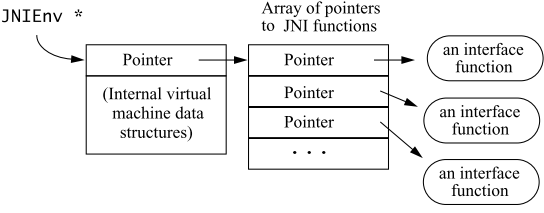
\includegraphics[width=12cm]{jni_function_table}
        \caption{JNI function table}
        \end{figure}
        \code{jobject} refers to the object that the method belongs. If it is a static method, it is a
        reference to the class that it belongs to. The \code{jstring} parameter is an argument given to
        the function in the Java code. In this case, it was a string passed into the method. There can be
        any arbitrary number of arguments passed into the function and will be reflected here when the C/C++
        function types are generated \citep{LiangJNISpecification}.

      \subsection{Performance}
        According to \cite{IBM2009} and \cite{WellsIPCMultiProc}, use of the JNI can incur
        performance penalties. Performance is somewhat restricted when calls to native code
        are made or when a JVM has to move up a class hierarchy. This is true if a native function
        attempts to call a method written in Java.

    \section{Linux and Solaris IPC Implementation}
      \subsection{Initial Implementation}
        A Linux and Solaris-based
        implementation was created by \cite{WellsIPCMultiProc} using Unix
        System V calls. The approach taken was to develop Java classes using JNI
        to access these system calls. The Unix IPC features used included
        message queues, semaphores, shared memory and piping. The
        implementation aimed to make the native Java methods as close to
        possible as the system calls. This includes names and parameter lists.

      \subsubsection{Problems Encountered}
        Problems encountered by \cite{WellsIPCMultiProc} was the
        difference in data representation between Java and C. Data representation
        issues arrised in aspects such as error handling (i.e. exceptions vs -1
        returns), control system calls, semaphore operations and shared memory.

      \subsubsection{Results}
        Simple communication was peformed and and
        compared against the network loopback connection. It was found that all
        the Unix System V IPC mechanisms were significantly faster than using the
        loopback method. Named pipes were found to be fastest since it made
        minimal use of JNI calls. This was the case for tests running on Ubuntu
        8.05.1 and Solaris.

      \subsection{Shared Memory Object Framework Model (SMOF)}
        The intial implementation by \cite{WellsIPCMultiProc} contained some
        portability issues since calls to native code were being made. A
        Shared Memory Object Framework (SMOF) was developed by \cite{WellsEfficientIPCJava} that aimed
        to create a more abstract solution to Java's IPC problems; thereby simplifying its porting
        to an OS such as Windows.

        The SMOF provides the programmer with classes that are used within shared memory. The objects of
        these classes act as an intermediary between data and the shared memory. Mutual exclusion is
        provided by means of Java monitor concepts. The primary class \code{SharedObject} is a parent
        class from which child classes are built. Two processes can access the shared object by using a
        key, which is essentially a file name that acts a point of reference \citep{WellsEfficientIPCJava}.

        \subsubsection{Results}
          Testing involved assessing the latency of sending simple messages between processes.
          The loopback approach and named pipes were used as benchmarks. It was found to be 80\% faster
          than named pipes and 87\% faster than the loopback network \citep{WellsEfficientIPCJava}.

    \section{Windows IPC and Concurrency Mechanisms}
      Modern Microsoft Windows Operating Systems appear to be highly modular in nature,
      with emphasis on object-oriented design which is illustrated by the following diagram taken from \cite{WinInt2009}.
      \begin{figure}[H]
      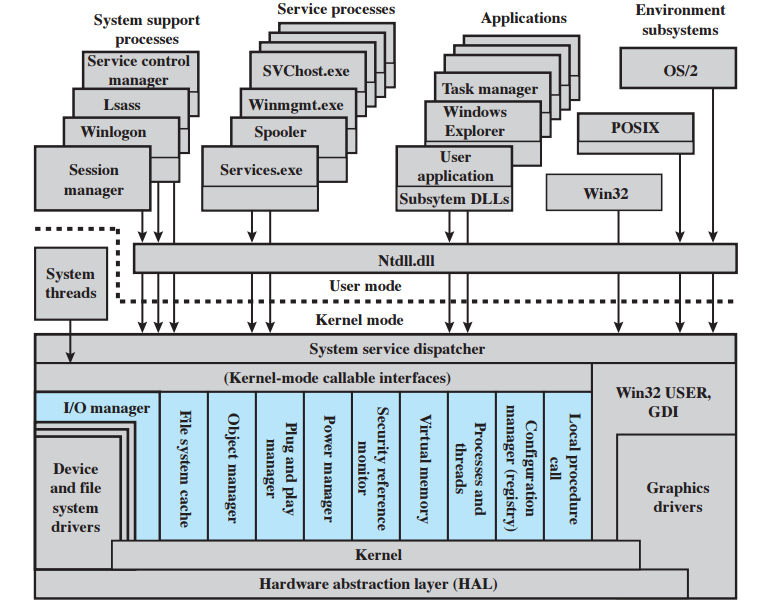
\includegraphics[width=10cm]{winArch}
      \label{fig:winArch}
      \caption{Windows System Architecture}
      \end{figure}
      According to \cite{OSInternals&DesignPrinciplesStallings}, the Windows kernel mode is
      divided into the following blocks: executive, kernel, the hardware abstraction layer,
      device drivers and the windowing and graphics system as depicted in figure 2.2 above.

      \subsection{Windows Executive}
        The Executive block contains the base services such as memory, thread management and IPC. The kernel block handles
        process switching and thread scheduling.
        It provides an application programming interface (API) for user mode software \citep{OSInternals&DesignPrinciplesStallings}.
        Within the Executive block, several other modules are built in. The module specific to IPC is the Process/thread manager.
        This module is responsible for creating, managing, and deletion of processes and associated threads.
        The Executive also contains a module called Local Procedure Call (LPC) that allows local processes to communicate.
        It is similar to remote procedure calls (RPC) \citep{OSInternals&DesignPrinciplesStallings}.
        The executive contains functions that are callable
        from user-mode through the Windows API \citep{WinInternalsPart12012}.

      \subsection{The Windows Process}
        Windows processes are defined as objects that have a number of attributes and functions
        (shown in figure 2.3) and contain at least one thread. These threads may execute in parallel on
        multicore systems. \citep{OSInternals&DesignPrinciplesStallings}.

        \begin{figure}[H]
        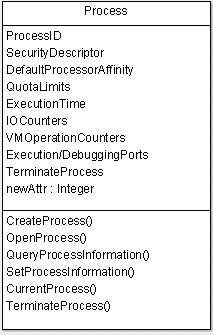
\includegraphics{procObj}
        \label{fig:procObj}
        \caption{A Windows process object. Taken from \cite{OSInternals&DesignPrinciplesStallings} p. 187}
        \end{figure}

        \subsubsection{CreateProcess()}
          The \code{CreateProcess()} function creates a process and its primary thread. The function takes the
          following parameters: the application name, command line to be executed, process attributes, thread attributes,
          inherit handles, creation flags, a pointer to the environment block, the current directory, start up information
          and current process information. The resulting process is assigned an identifier and is
          valid until termination. \code{TerminateProcess()} can be used to the kill the process by
          passing in the correct handle to the process that needs to be exited. Additional functions
          exist in the Windows API that complement this function and include functionality such as returning
          handles, opening processes, returning process information and so forth \citep{MSDN_API}.

      \subsection{Windows' Client/Server Model}
        Windows' services, subsystems and IPC mechanisms are structured according to a client-server model of
        computing which aims to simplify the Executive, improve reliability and provide a base for distributed
        computing \citep{OSInternals&DesignPrinciplesStallings}. Windows' IPC mechanisms are abstracted by means
        of this model where a client is a process that requests data from another process. A server responds to
        such requests \citep{MSDN_IPCExplanation}. The following subsection discusses how applications can communicate.

      \subsection{Process Communication Mechanisms}
        Windows provides the following IPC mechanisms as per the APIs provided by Microsoft (Windows API).

        \subsubsection{Clipboard}
          The clipboard acts as a depository which allows applications to share data. An application
          deposits data into the clipboard which another application can later retrieve in a format it understands.
          Applications can be running on the same machine or across a network. Clipboards are user driven and should
          only send data upon a user command and not in the background (i.e. not without the user's knowledge). The
          clipboard represents a single central depository which multiple other applications can access, as such a
          process cannot create its own clipboard. \citep{MSDN_IPCExplanation}.

          Key functions such as \code{OpenClipboard}, \code{EmptyClipboard}, \code{SetClipboardData},
          \code{CloseClipboard} and \code{GetClipboardData} are used \citep{IPCWindowsLinkedInSlides}.
          \code{SetClipboardData} deposits data on the clipboard in a particular format.
          \code{GetClipboardData} retrieves data from the clipboard in the format specified \citep{MSDN_API}.

        \subsubsection{Component Object Model (COM)}
          The Component Object Model can be used to create software components that can interact.
          According to \cite{MSDN_API}, it is a standard that defines how COM objects interact with other
          objects. Objects can reside in a single process or in multiple other processes. COM objects can
          access data and an object's data through a set of functions known as interfaces. The functions that
          are part of the interface are known as methods. Interface methods are accessed through a pointer to
          that interface. Common functions exist between all COM objects; i.e. they are mandatory
          functions that all components require.

        \subsubsection{Data Copy}
          By making use of \code{WMCOPYDATA} that is part of Windows Messaging, an application can
          send data to another application. In order to use data copying, the receiving process needs
          to be aware of the format of the data being sent as well as identity of the sending process.
          Data can be encapsulated within a private data structure. It can be sent to the receiving application
          along with the a pointer to the data structure using \code{WMCOPYDATA} \citep{MSDN_API}.

        \subsubsection{Dynamic Data Exchange (DDE)}
          \cite{MSDN_API} defines DDE as an extention of the Clipboard as it makes use of the same formats.
          Data can be exchanged at an ongoing rate, or as new data becomes available. \cite{MSDN_API} desribes
          DDE as not as efficient as newer IPC mechanisms. Its important to note that the DDE makes use of shared
          memory to exchange data between appilcations.

          DDE contains a .dll file called Dynamic Data Exchange Management Library (DDEML) that processes
          can use to share data. The library provides functions and messages that adds DDE to applications.
          DDEML makes use of a conversation concept that makes it easier for the programmer to manage messages; pointers and atomic access to
          shared memory are replaced by making use of string handles. In addition, DDEML forces applications to implement DDE in a
          consistent fashion. Programs should have the DDEML header file within its source code \citep{MSDN_API}.

          A DDE client can start a conversation with a DDE server and can participate in multiple conversations
          simultaneously. A process can be a client or a server as necessary. DDE conversations are identified by
          the process/application name and a ``topic". The topic represents the data that is to be exchanged between
          processes \citep{MSDN_API}.

        \subsubsection{File Mapping}
          File mapping allows a process to see the contents of a file as a block of memory within its own address space.
          This is essentially a form of shared memory. Pointer operations are used to access and modify contents of the
          mapped file with some form of synchronisation mechanism (such as a semaphore) used to prevent corruption and
          maintain the file's consistency. This IPC technique can only work on a single machine and the file cannot exist
          on a remote computer \citep{MSDN_API}.

          \cite{IPCWindowsLinkedInSlides} states that a file mapping can be created by using the function \code{CreateFileMapping}.
          The file map view is then put into address space of the current process by using \code{MapViewOfFile}. \code{CopyMemory} is
          then used to write messages to the view. File mappings are closed using \code{UnmapViewOfFile} and \code{CloseHandle}.
          A client process can examine the contents of the mapping using \code{OpenFileMapping} and put the view into its address
          space by calling \code{MapViewOfFile}. It can also close mappings as necessary.

        \subsubsection{Mailslots}
          Windows Mailslots follow the client-server model with one-way process communication. A server process will create a Mailslot
          and the client can write messages into the Mailslot as required. The messages are saved within the Mailslot until read.
          Messages can be sent on a local host or across a network. Message size is only limited by what the server specifies when
          the slot is created \citep{MSDN_API}.

          Mailslot messages follow a datagram format and as such, no guarantees are made in terms of receipt. Mailslots receive a
          handle when created which is used when the process that created it accesses data within it. A process that is aware of a
          Mailslot's existence can insert a message there. Mailslots also have a broadcasting capability where each process can
          create a slot and all participating processes can deposit their messages to the respective Mailslots that exist. This
          means that a Mailslot can be a server and client which can allow two-way communication \citep{MSDN_API}.

          Mailslots can be created using \code{CreateMailslot()} and its contents examined using \code{ReadMailslot()}. A number of
          auxiliary functions exist such as \code{GetMailslotInfo()} and so forth. Handles can be closed using \code{CloseHandle()}.
          Clients can create a file and write to the slot using \code{CreateFile()} and \code{WriteFile()}/\code{WriteMailslot()}
          \citep{IPCWindowsLinkedInSlides}.

        \subsubsection{Pipes}
          Windows uses two types of pipes for IPC: anonymous and named pipes.

          Anonymous pipes only allow related processes to exchange data and cannot be used over a network.
          They are typically used to exchange data between parent and child processes by using read and write
          handles respectively. \code{CreatePipe()} returns read and write handles for an anonymous pipe and
          specifies a buffer size. These handles are passed to another process to communicate, usually by means of
          inheritance where the handle is passed from the parent (server) process to the child (client) process.
          The relevant handle is sent depending on whether a read or write operation must occur. \code{ReadFile()}
          is used to read from the pipe and conversely \code{WriteFile()} is used to write to the pipe.
          \code{CloseHandle()} closes a process's pipe `connection' \citep{MSDN_API}.
          Asynchrony is not supported by anonymous pipes \citep{lewandowski1997interprocess}.

          According to \cite{MSDN_API}, named pipes can be used between unrelated processes and across a network.
          Processes can act as a server or client without having to create multiple anonymous pipes.
          \code{CreateNamedPipe()} and \code{ConnectNamedPipe()} are used by the server and client respectively.
          Standard \code{ReadFile()} and \code{WriteFile()} functions read and write to the pipe as necessary.

        \subsubsection{Remote Procedure Call (RPC)}
          Similar to RMI discussed above, RPC allows procedures to be called remotely, either on a
          local machine or across a network. \cite{MSDN_API} states RPC conforms to the Open Software
          Foundation's (OSF) Distributed Computing Environment (DCE) which allows RPC to work on other
          OSs that support DCE.

        \subsubsection{Windows Sockets (Winsock 2)}
          Winsock creates a channel between communicating processes and is protocol independent with
          asynchronous communication capabilities \citep{lewandowski1997interprocess}. Socket handles
          can be treated as a file with usual I/O operations \citep{MSDN_API}.

          Data communicated by processes can be stream-based in the form of bytes or packetised in the form
          datagrams but no quality of service is guaranteed \citep{IPCWindowsLinkedInSlides}. In terms of local IPC,
          localhost can be used to send and receive data, as long as the correct IP addresses are specified.

      \subsection{Windows Interprocess Synchronisation}
        The Windows API provides functions that allow processes to synchronise as necessary. This is particularly
        important with regards to shared memory when there is competition for resources. Functions such \code{CreateEvent()},
        \code{CreateSemaphore()}, \code{CreateMutex()} among others return handles that processes can use for the same event.
        These are generally used in conjunction with the security parameter defined in \code{CreateProcess()} \citep{MSDN_API}.

    \section{IPC in Mac OS X and Generic Considerations}

      \subsection{Mac OS X}
        Mac OS X generally treats other processes as hostile to enforce security mechanisms in its IPC design.
        IPC mechanisms used are Mach Messaging, Distributed Objects, Shared Memory and Signals \citep{MAC_API}.

        \subsection{Generic Considerations}
          Microsoft Windows, Linux-based OSs with many flavours and Mac OS X are the most popular and most well-known OSs.
          As such generic considerations should be made. In terms of IPC, a common form of IPC would be shared memory.
          From the review conducted above, shared memory is common to the three and can provide a reasonably efficient
          method in which to implement IPC (as illustrated by SMOF). A generic version could be developed that utilises
          hese concepts and suitably abstracts away OS dependencies.

          Since a Linux version of Java IPC has been developed by \cite{WellsIPCJava}, and subsequent to the
          windows implementation proposed, future work could be completed in achieving a Mac OS version.
          A generic design then could be implemented that would aim to be OS independent.

      \section{Chapter Summary}

        The current trend of multicore computing emphasises the significance of parallelism, multithreading and
        communication in general \citep{taboada2013javaforHPC}. It is important to utilise these concepts to make
        software scalable \citep{SlinnJVMAkka}.

        Investigation of Java's concurrency mechanisms found that the language is heavily thread
        oriented and that it provides a good mechanism for multithreading programming. Opposed to this is the
        language's lack of communication between separate JVM processes.

        The existing Linux and Solaris implementation that used JNI to provide Java with IPC was successful and
        proved that a more efficient method of IPC could be developed without using the loopback method and ``clunky"
        socket programming. The review of the use of JNI highlighted a few efficiency problems with calls to native code,
        therefore calls to JNI should be as limited as possible. In addition, the SMOF proved that portability issues can be
        addressed, but it may limit IPC communication to shared memory. As such, use of common IPC features among different OSs
        should be taken into account when developing a generic version of the Java class library.

        Windows provides a fairly comprehensive set of IPC mechanisms that can be integrated with Java processes,
        albeit at the cost of complexity when compared to Unix system calls.

        Mac OS X provides mechanisms that are common to Windows and Linux; namely shared memory.
        This can definitely be considered as a goal to aim for in terms of a generic solution to this problem.

  % CHAPTER 3
  \chapter{Project Approach}
    % GIVE A GENERAL OVER VIEW OF THE CHAPTER HERE ONCE IT IS COMPLETE
    % POSSIBLY MENTION SOMEWHERE IN THIS CHAPTER WHY I DIDN'T DO  SOME THING-E.G. CLIPBOARD, ANON PIPES ETC
    The following chapter provides a broad, high-level view of the methodologies used during the
    design and implementation phase of the project.
    \\\\
    Section \ref{hardwareused} discusses the hardware that was used for the project.
    Section \ref{softwareused} discusses the software and other related technologies that were used
    during development as well as the results phase of the project. This includes critical software
    required by the system as well as other non-critical software that supplemented the development process.
    Section \ref{devapproach} discusses broadly how I designed and implemented the actual system. It outlines the
    order in which I implemented each Windows IPC mechanism, why this was the case and any benefits this
    may have yielded. Finally, section \ref{results} discusses the methodology used to collect and analyse results.

    \section{Hardware} \label{hardwareused} % hardware used in the project
      I used one primary desktop machine for the majority of the project's development. It had the following specifications:
        \begin{itemize}
          \item Intel Core i5-6400 Quad-Core CPU @ 2.70 GHz.
          \item 8 GB DDR3 RAM.
          \item WDC 400 GB HDD.
          \item Intel HD Graphics 530 with 4 116 MB VRAM.
          \item Windows 10 Enterprise 64 bit Insider Preview Build 14393.
        \end{itemize}
      In addition, a secondary machine was used for development and testing purposes:
        \begin{itemize}
          \item	Intel Core i3-2350 Quad-Core Sandy Bridge CPU @ 2.30 GHz.
        	\item	4 GB DDR3 RAM @ 655 MHz.
          \item WD 1 TB HDD
        	\item NVIDIA GeForce GT 520MX GPU with 1024 MB VRAM.
          \item Windows 10 Home 64-bit Build 10856.
        \end{itemize}

    \section{Software} \label{softwareused}% software used in the project
      Various software packages were used for the project, including critical and
      non-critical support packages.
        \subsection{Critical Software}
          Since the project's focus is on IPC mechanisms on a Microsoft Windows
          platform, it is palpable that a Microsoft Windows operating system was used. As described in
          Section \ref{hardwareused}, two versions of 64 bit Windows 10 were used on two separate
          machines during the implementation and testing phases of the project. I consciously made
          the decision to develop on Windows 10 because it generally provides
          consistent backwards compatibility \citep{win10BC}. The Windows API is also fully supported
          by Windows 10 OSes \citep{MSDN_API}. In addition, I thought using Windows 10 made the most sense
          since it is Microsoft's latest OS product. In addition, I wanted to install the Windows 10 Insider Preview
          to test Bash On Ubuntu On Windows \footnote{https://msdn.microsoft.com/en-us/commandline/wsl/about} (which will be discussed later in this text).
          \\\\
          Another fundamental software component of this project is the Java Development Kit. I made
          use of the Java SE Development Kit 7 \footnote{http://www.oracle.com/technetwork/java/javase/downloads/jdk7-downloads-1880260.html} or JDK 7 as a 32 bit Java Virtual Machine (JVM).
          This includes the standard Java APIs as well as the required header files needed to
          make use of the Java Native Interface. I initially installed a 64 bit version of the JDK and
          immediately encountered problems in terms of code compilation with programs that used native
          C code. Upon compilation, my test programs were unable to load the native library and a
          \code{UnsatisfiedLinkError} exception occurred, outlining that it could not load a 32 bit .dll
          on a 64 bit Java platform. The solution to this was to install a 32 bit JDK (and hence 32 bit
          JVM) and recompile.
          \\\\
          In order to compile the native C code that accesses Windows' IPC mechanisms, a C or C++
          compiler was needed. Since the project is on a Windows platform, the clear choice was the
          Microsoft Visual C++ compiler \footnote{https://www.microsoft.com/en-us/download/details.aspx?id=41151}.
          It integrates with Microsoft's Visual Studio Integrated
          Development Environment (IDE) products but can also be called from the command line by
          executing \code{cl.exe} in the Visual C++ directory, located in Windows' Program Files file structure.

        \subsection{Non-critical Software}
          The fundamental support package used throughout this project was GitHub. This served
          as my version control throughout the implementation of each IPC feature. I made use
          of a Git GUI client called GitKraken\footnote{https://www.gitkraken.com/}.
          \\\\
          JUNIT\footnote{http://junit.org/junit4/} is a Java library that provides a unit testing framework. This
          was used to ensure that Java methods performed as expected.
          \\\\
          The programming language R\footnote{https://www.r-project.org/} was used in the analysis phase of the project, along with Microsoft Excel 2016.
          The R source code I developed is available with WindowsIPC on the JavaIPC GitHub repository.
          \\\\
          Atom was the code editor used throughout the development and testing process.

    \section{Design Approach and System Overview} \label{devapproach}
      The first phase prior to implementation was to become familiar with
      the JNI framework. This involved designing simple JNI programs to become competent
      in terms of how primitive data types are handled, how parameters are passed, how memory is
      allocated and freed and how values are passed between the JVM and native C code.
      For example, since Java uses UTF-16 strings that are passed down into the JNI, they
      have to be fetched using \code{GetStringUTFChars} which allocates them to a pointer and converts
      them to UTF-8. They then have to be released using \code{ReleaseUTFChars} since the memory
      is not freed upon function return \citep{Android}. Throughout this process,
      I followed \cite{LiangJNISpecification} which provided well structured and easy to understand
      JNI examples and tutorials, which greatly aided in the understanding of JNI. This was fundamental
      during the implementation of WindowsIPC since a thorough understanding of how JNI works was needed
      to ensure the stability and usability of the system. Concurrent to this, I cemented my C coding ability since
      a significant majority of time was spent developing in C. I also ensured I knew how to compile and build Java programs
      that used JNI. This involved understanding the various flags and include files that needed to be added to the command line.
      As such, I decided to build the system using the command line and not an IDE. As such I made use of Windows Batch scripts that
      specified system dependencies and files that were needed to compile and execute the code. Listing 3.1 is a
      snippet of a batch script that generates files required by the system. I preferred to develop in a
      simple code editor as I found that initialising an IDE to use JNI was rather tedious and not worth the time. In addition,
      complex debuggers would not have been beneficial since parallel development is notoriously difficult to debug.

      \begin {lstlisting} [caption=Batch Script Snippet]
        REM create the header file
        "C:\Program Files (x86)\Java\jdk1.7.0_79\bin\Javah" -jni -classpath
        "C:\Users\g13s0714\Desktop\CS Honours\GitHub\JavaIPC\Implementation"
        WindowsIPC
      \end{lstlisting}

      Once I had gained suitable confidence with using JNI to access native C code,
      I ranked each Windows IPC mechanism in terms of ease of implementation based on research conducted
      in terms of their use in other systems. This involved understanding
      the related WINAPI functions. I believe this was a logical method to follow that made the development
      process significantly easier. I started developing Java Sockets since this is the only method of
      IPC that Java offers (as mentioned in Chapter 2). In addition, I wanted to
      use this as a benchmark to determine if the other mechanisms perform better.
      This involved timing message sending between two Java programs that made use of
      the socket.
      \\\\
      % PARAGRAPH WILL BE EDITED ONCE I HAVE COMPLETED DEVELOPMENT
      Once I had a suitable benchmark from developing Java Sockets, I proceeded with the development of
      the Windows IPC mechanisms. Windows typically implements IPC using a client-server model which
      I conformed to during my implementation. I first implemented Named Pipes, followed by Mailslots, Windows Sockets,
      Windows File Mapping (a shared memory equivalent) and finally Data Copy. This entailed analysing and understanding the
      relevant WINAPI functions that were necessary for their implementation. I found that most of Microsoft Windows' APIs were significantly
      complex and difficult to understand. This was apparent in the many function parameters and flags that are present
      in WINAPI functions. I also found that most of the function examples on the Microsoft Developer Network were given in C++ code,
      which was problematic since WindowsIPC was written in C. As a result, C and C++ syntax is used interchangeably. Ultimately, this did not
      pose any significant problem, since Visual C++ could handle it's compilation.
      \\\\
      Figure 3.1 presents a graphical, high-level overview of the system. It illustrates the problem that two Java programs cannot
      communicate within the ``Java World" but can in the ``native C/C++ World".
      through the use of JNI. The actual communication is done by making use of
      WINAPI functions which can call the relevant IPC function(s). This
      allows the system to feed messages back and forth between the Java and C/C++ levels.
      Note: the term ``coordination" refers to both synchronisation and communication.

      \begin{figure}[H]
        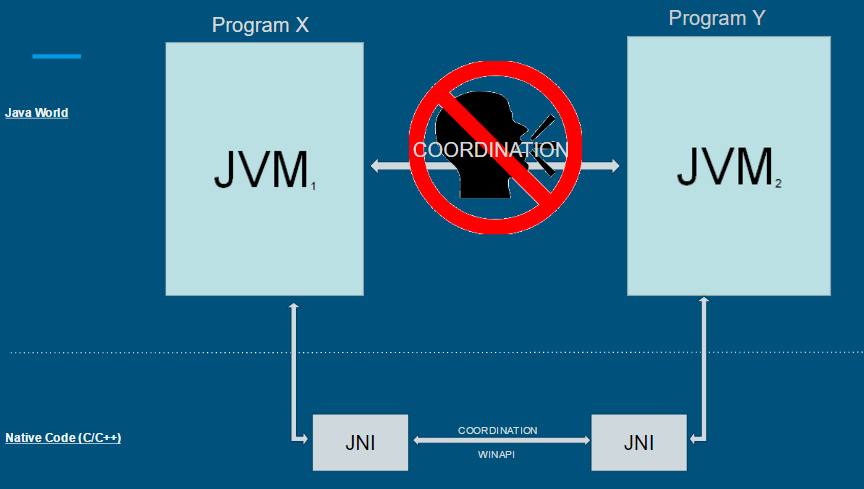
\includegraphics[scale=0.7]{SystemOverview}
        \label{fig:SystemOverview}
        \caption{High-level Overview of WindowsIPC}
      \end{figure}


      During the implementation of each feature, I tested it by writing small Java test programs that used the native code to send
      messages to each other. Messages sent were simple byte arrays. The size (in terms of the number of elements)
      of the array sent were simply hardcoded as 40, 400, 4 000 and 40 0000. For example, a byte array with 400
      elements represents a message size of 400 bytes. Two Java test programs (for each mechanism) were used to ensure that messages were sent between two
      distinct Java processes. Following this, I wrote a single Java program for each mechanism that used \code{java.util.concurrent} to create a thread
      that communicated with the program's main thread. This was achieved by implementing the \code{run} method of the \code{Runnable}
      interface. The \code{run} method uses an object of WindowsIPC to call method to send a message to the program's main thread. This was done
      to ensure true communication was possible (i.e. between separate processes as well as threads executing within a single JVM instance).


      % DISCUSSION OF HOW I WENT ABOUT RESULTS ANALYSIS
    \section{Results Analysis} \label{results}
      In order to time the execution of each native method as well as the Java Sockets execution time, I used the following Java code:
      \begin {lstlisting}[caption=Java Timing Code]
        long time = System.nanoTime();
          //Method being timed goes here...
        System.out.println("Time to get message from file mapping: "+ ((System.nanoTime() - time))+ "ns");
        System.out.println("Message in Java: " + x);
      \end{lstlisting}

      For each message size, I timed the execution of the method that sent the actual message 10 times and then calculated a mean execution time. I
      used this figure to determine a speedup in comparison to Java Sockets to illustrate the performance gain
      that was achieved. Each timing value was copied into an R script that calculated the mean for the relevant IPC mechanism.
      I also made use of Microsoft Excel to provide a convenient method in which to view results without having to scan through an
      R script file. Once the mean execution time for each mechanism was calculated, the R script generated various graphs, including line and
      bar graphs. This provided a graphical way in which to display each mechanism's performance relative to Java Sockets. Listing 3.3 shows R
      code that calculates the mean execution time of Java Sockets in micro-seconds for each byte size and then generates a line graph
      illustrating the relationship.

      \begin {lstlisting}[caption=Snippet of R Script that Generates Stats and Graphs]
        JS_VECTOR <- c(
        JSOCKETS_40_BYTES / 1000,
        JSOCKETS_400_BYTES / 1000,
        JSOCKETS_4000_BYTES / 1000,
        JSOCKETS_40000_BYTES / 1000
        )
        png(file = "JavaSocketsLineChart.png")
        plot(
          JS_VECTOR,
          col="red",
          xlab="Size of Message in Bytes",
          ylab="Time to Send in MICRO-SECONDS",
          main="Java Sockets Performance",
          type='b',
          xaxt="n",
          ylim=c(6000, 6400)
        )
        axis(side=1, at=1:4, lab=c("40","400","4 000","40 000"))
        dev.off()
      \end{lstlisting}

      The graphs generated aided in the discussion chapter of this text due to the visual illustration of the results.
      It showed the excellent speed up that can be achieved by making use of this library as opposed to the use of a
      socket mechanism. The results obtained are discussed in \ref{resultsch}
      % SUMMARISE HERE ALL THE SECTIONS THAT DISCUSS WHAT WHEN FINISHED



  % IN DEPTH DISCUSSION OF EACH WINDOWS IPC METHOD
  \chapter{Implementation of Windows' IPC Mechanisms}
    \section{Introduction}
      This chapter presents an in-depth discussion of the implementation of WindowsIPC. It includes a thorough
      discussion of the design methodology, problems that were encountered as well as the relative success or lack
      thereof of each IPC mechanism. In addition, discussion centers around the various WINAPI functions used and
      why this was the case. Section \ref{syscomp} discusses system compilation and file generation. It includes
      a discussion of the build script that was developed as well as the files generated by the system.

    \section{Files, File Generation and System Compilation} \label{syscomp}
      \subsection{System Files}
        \begin{itemize}
          \item WindowsIPC.java
          \item WindowsIPC.C
          \item make.bat
          \item clean.bat
          \item run.bat
          \item WindowsIPC.dll (System generated)
          \item WindowsIPC.h (System generated)
          \item WindowsIPC.obj (System generated)
          \item WindowsIPC.lib (System generated)
          \item WindowsIPC.exp (System generated)
        \end{itemize}

        The primary Java file for this system is called \code{WindowsIPC.java}.
        This class contains all the native methods and support methods that are needed for the implementation
        of the system. The system is designed in such a way that users can declare an object of the class
        WindowsIPC and use it to invoke the relevant IPC functions depending on the needs of the application.

        The C file that contains the implementation of the JNI functions is of the same name:
        WindowsIPC.c. WindowsIPC.h is system generated and contains the function prototypes which are implemented in
        WindowsIPC.c. The majority of implementation was done in WindowsIPC.c, with tests conducted in small Java
        programs.

        A number of files are system generated and hence not implemented directly. These are namely the files required
        to access Windows' APIs.

      \subsection{File Generation and System Compilation}
        As mentioned in Chapter 3, I did not make use of an IDE throughout the implementation phase of this
        project, but instead used Windows Batch Scripts to build the system and generate the required files.

        % ADD REFERENCE HERE ABOUT 32 BIT VERSUS 64 BIT CONFLICT ()
        % discuss point of vcvarsall.bat
        The primary batch script that I developed is called make.bat. This script performs
        the initial file generation and Java compilation. It generates the native library called
        WindowsIPC.dll that the JVM loads to make use of the JNI functions defined in WindowsIPC.h
        and implemented in WindowsIPC.c. It is important to note that since this script defines directory locations
        that are specific to the two machines that were used for development, it will not work on any other
        additional machines without significant modification. The script initially changes the working directory
        to the local GitHub repository directory that contains the files of the system. This is performed using a simple
        \code{cd} command. It then calls the vsvarsall.bat batch script that sets up the environment variables
        of that particular terminal session. This script configures the command line for 32 bit or 64 bit compilation and comes standard
        with a Microsoft Visual Studio installation. This is required to make use of cl.exe (the Visual C++) compiler.
        When calling vcvarsall.bat, ``x86" is passed in as an argument to force the system to be used within a
        32 bit context. This prevents any 32 bit versus 64 bit conflicts (as discussed in Section \ref{softwareused})
        when used in conjunction with a 32 bit JVM.\citep{ENVBUILDS}.
        The script then compiles WindowsIPC.java using the Java compiler (\code{javac}) followed by generating
        WindowsIPC.h. This is done by executing \code{javah} and specifying the classpath of WindowsIPC.java
        (i.e. the location of the .class file). Following the generation of WindowsIPC.h, \code{cl} is
        executed. To run this command and to integrate it successfully with Java's JNI, the correct
        include directories that contain the required header files needed for
        the generation of the native library must be specified. This is achieved by using the \code{-I} flag
        and then specifying the location of the win32 header files as well as the header files needed by the JNI.
        The \code{-LD} flag is used to specify WindowIPC.c and \code{-FE} specifies the name of the native library (i.e.
        the name of the .dll file generated by \code{cl}).
        In addition, this command generates .lib, .exp and .obj files of the same name.
        These files are required to access the Windows API. % REF THERE PURPOSE HERE
        WindowsIPC.java is then executed to ensure that it was correctly
        compiled and that all the required files were generated successfully.

        An additional script called clean.bat simply deletes all generated files. It uses a simple \code{del}
        command to delete the files with a specific extention. For example, \code{del *.class}
        deletes all generated class files and \code{del WindowsIPC.dll} deletes the generated native library.

        The script run.bat simply executes WindowsIPC.java by calling the Java interpreter \code{java}.
        This was written to perform a quick execution of WindowsIPC and hence prevent the need to rebuild
        the entire system.

        WindowsIPC.java loads the native library (WindowsIPC.dll) generated by \code{cl} by using the following Java syntax:
        \begin {lstlisting}[caption=Loading The Native Library]
          static {
            System.loadLibrary("WindowsIPC");
          }
        \end{lstlisting}
        ``WindowsIPC" is the name of the .dll file that contains the required native functions. This code
        is specified outside of any method within the Java file, hence it is defined as a static code block.
        This is performed below the declaration of the native functions.
        % CHECK IF LIBRARY REALLY MUST BE LOADED BELOW NATIVE METHOD DECLARATION


    % should add some references here used during implementation --> i.e. tutorials used etc
    \section{Java Sockets} \label{jsockssections}
      The implementation of Java Sockets does not contain any use of the JNI and simply is implemented
      as standard Java methods in WindowsIPC.java. Since this
      implementation is making use of Java's networking capabilities,
      the \code{java.net} package needed to be imported. This is necessary to create objects such as
      \code{ServerSocket} and \code{Socket} object and other networking-related objects \citep{JavaAPI}.
      There are two method implementations, one represents
      the socket server and another that represents the socket client. This aims to conform to Windows' client-server
      model of IPC implementation.

      The server method is designed in such a way that
      it allows a client to connect to it, then pass data to it as it likes. The method then simply returns
      the client message as a byte array. The method is called \code{createJavaSocketServer} that takes a port number as an argument.
      Some error checking is in place that ensures the port number is valid and unprivileged.
      If an invalid port number is passed in, an error is raised.
      Otherwise, a \code{SocketServer} object is created that passes the port number into its constructor.
      Then a \code{Socket} object is created and initilised by calling \code{accept} on the original
      \code{ServerSocket} object, as depicted in Listing 4.2. The \code{accept} method waits
      for a client connection.

      \begin {lstlisting}[caption=Java Sockets: \code{createJavaSocketServer}]
        public byte[] createJavaSocketServer(int port) {
          byte[] messageRcv = null;
          ServerSocket serverSocket = new ServerSocket(port);
          Socket server = serverSocket.accept();
          DataInputStream in = new DataInputStream(server.getInputStream());
          int length = in.readInt();
          messageRcv = new byte[length];
          if (length > 0)
            in.readFully(messageRcv, 0, messageRcv.length);
          server.close();
          // some excption handling...
          return messageRcv; // return the message sent from the client
        }
      \end{lstlisting}

      A \code{DataInputStream} object, called \code{in} is created. This object is used to extract the message
      sent by the client from the socket connection. It does this by invoking \code{getInputStream}
      using the \code{Socket} object.
      A byte array called \code{messageRcv} is declared which is used to store the message
      received from a client connection. The size of the array is specified by determining the
      length of the message received using \code{in} and calling \code{readInt} on it.
      If there is a message, then \code{readFully} gets the message and dumps it into the
      the byte array. The server is then closed and the byte array message is returned.
      All of this code is wrapped in a try-catch block. It catches any \code{IOExceptions}
      that may be raised. It has been omitted from Listing 4.2.
      \\\\
      The Java Socket client was implemented in Java method called \code{createJavaSocketClient}.
      This method returns an integer value that represents whether the method executed as expected or not.
      A returned value of zero indicates that the method executed as expected.
      -1 indicates an error occured. The method takes the host name, port
      and message as arguments. The host name, in this case, should always be localhost (127.0.0.1).
      The port number should be above 1024 to ensure privileged port numbers are not used. The programmer who makes
      use of this method should specify 127.0.0.1 and the port number that was specified when the server was
      created. The message parameter is a simple byte array. To create the client, an object of \code{Socket}
      called \code{client} is created. This object is instantiated by passing loopback and the port number to the
      \code{Socket} constructor. An \code{OutputStream} object is instantiated by invoking \code{getOutputStream}
      on \code{client}. This is the primary output stream that is used to send the byte array message to the
      server. This is achieved by passing this object to a new \code{DataOutputStream} object's constructor. This
      object is called \code{out}. The actual message is sent by
      using \code{write} which called on \code{out} and takes the message as an argument.
      The client is then closed. If any error is occured (such as an \code{IOException}), then -1 is returned,
      otherwise zero is returned which indicates the method successfully sent the message to the existing
      server application. This method also includes some exception handling code, which is required when using
      \code{Socket} objects. This process is illustrated in Listing 4.3 below. Note: It also omits the exception
      handling code.

      \begin {lstlisting}[caption=Java Sockets: \code{createJavaSocketClient}]
        public int createJavaSocketClient(String host, int port,
                                          byte[] message)
        {
            Socket client = new Socket(host, port);
            OutputStream outToServer = client.getOutputStream();
            DataOutputStream out = new DataOutputStream(outToServer);
            out.writeInt(message.length);
            out.write(message);
            client.close();
            return 0; // success
        }
      \end{lstlisting}

      Overall, the implementation of Java Sockets using \code{Socket} objects was
      relatively straightforward, with little difficulty. 



    \section{Named Pipes} \label{npsection}

    \section{Anonymous Pipes} \label{anonpipesection}

    \section{Mailslots} \label{mssection}

    \section{Windows Sockets} \label{winsocksection}

    \section{File Mapping} \label{filemapsection}

    \section{Data Copy} \label{datacopysection}

    \section{Dynamic Data Exchange} \label{ddesection}

    \section{Clipboard} \label{clipboardsection}

    \section{Component Object Model} \label{comsection}

  \chapter{Results} \label{resultsch}

  \chapter{Discussion}

  \chapter{Conclusion}

  \addcontentsline{toc}{chapter}{References}
  \bibliographystyle{ruauthordate}
  \bibliography{refs2}

\end{document}
